\section{\I{The population section}\label{sec:population-section}}

\subsection{Introduction}
The population section\index{Population section} specifies the model structure, population dynamics, and other associated parameters. It describes the model structure (population structure), defines the population processes (e.g., recruitment, migration, and mortality), selectivities, and their parameters.

The population section consists of several components, including;
\begin{itemize}
  \item The population structure;
  \item Model initialisation (i.e., the state of the partition at the start of the first year)\index{Initialisation}\index{Model ! initialisation};
  \item The years over which the model runs (i.e., the start and end years of the model)
  \item The annual cycle (time-steps and processes that are applied in each time-step)\index{Annual cycle};
  \item The specifications and parameters of the population processes (i.e., processes that add, remove individuals to or from the partition, or shift numbers between ages and categories in the partition);
  \item Selectivities;
  \item Parameter values and their definitions;
  \item Derived quantities, required as parameters for some processes (e.g. Mature biomass to resolve any density dependent processes such as the spawner-recruit relationship, in a recruitment process).
\end{itemize}

\subsection{\I{Population structure}}

The basic structure of population section of a \CNAME\ model is defined in terms of an annual cycle, time steps, states, and transitions.

The annual cycle defines what processes happen in each model year, and in what sequence. \CNAME\ runs on an annual cycle rather than, for example, a 6-monthly cycle.) 

Each year is split into one or more time steps, with at least one process occurring in each time step. Each time step can be thought of as representing a particular part of the calendar year, or you can just treat them as an abstract sequence of events. In every time step, there exists a mortality block, this is a block (a group of consecutive processes) where individuals are removed from the partition. If there are no mortality processes then the mortality block is empty (nothing happens) and occurs at the end of a time step. \CNAME\ will error out if the user defines multiple mortality processes in a single time step, that are not consecutive processes.

The state is the current status of the population, at any given time. The state can change one or more times in every time step of every year. The state object must contain sufficient information to figure out how the underlying population changes over time (given a model and a complete set of parameters).

There are a number of possible changes in the state, which are called transitions. These include processes that include recruitment, natural mortality, anthropogenic mortality, ageing, migration, tagging events, and maturation. Different processes may be useful for different models in different circumstances.

The division of the year into an arbitrary number of time steps allows the user to specify the exact order in which processes and observations occur throughout the year. The user needs to specify the time step in which each process occurs. If more than one process occurs in the same time step, they will be applied in the order specified in the \command{time\_step} block.

The key element of the state is the partition. This is a broadly applicable concept that can be used to describe many different kinds of population model. The partition is simply a breakdown of the total number of individuals in the current population into different categories. (Note that the partition records numbers of individuals, not biomass). The individuals are grouped into categories, for example, sex, maturity state, area, and species. However \CNAME\ has no predefined categories, and these are defined by the user. This differs from CASAL \citep{1388} that has only pre-defined partition categories. 

The resulting partition can be conceptualised as matrix, where each row is represented by a category and the columns are the age classes, shown in Figure~\ref{Fig:part}. Each row represents the number of individuals for that category in that age class. 
	
The names of categories are user defined, and there must be at least one category defined for a model. The ages are defined as a sequence from $age_{min}$ to $age_{max}$, with the last age optionally a plus group. In order to calculate biomass, the age-length relationship for each category must also be defined for an age based model (but could be defined as `none'). An example of how this is specified for four categories based on sex and area is as follows,
{\small{\begin{verbatim}
	@categories 
	format mature.sex 
	names 		spawn.male 	spawn.female 	nonspawn.male 	nonspawn.female
	age_lengths 	male_AL		female_AL   male_AL		female_AL  
		\end{verbatim}}}	

For an example of these ideas, consider a model of a fish population with a mature and non-spawning fishery. If we assume that the non-spawning fishery happens over most of the year (say 10 months) in the non-spawning area. The mature fish then migrate to the spawning area, where the spawning fishery operates. At the end of spawning, these fish, along with the recruits from the previous year, migrate back to the non-spawning area. The modeller decides that fish will be divided in the partition by age, sex, maturity, and area (spawning and non-spawning grounds). So the partition has 8 rows (2 sexes × (mature or immature) × 2 areas) and one column per age class. 

\begin{figure}[H]
	\centering
	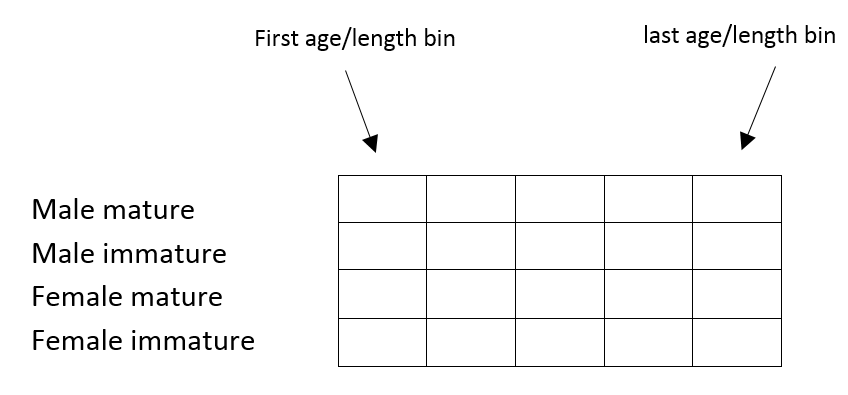
\includegraphics[scale=0.3]{Figures/partition.png}
		\caption{A visual representation of a partition}\label{Fig:part}
\end{figure}

So they define four time steps, labelled 1 through 4. Step 1 includes the non-spawning fishery. Step 2 includes the migration to the spawning area. Step 3 includes the spawning fishery. Step 4 includes recruitment and the migration back to the non-spawning area. (In fact, they could have used only 3 time steps, by using a single step in place of their steps 2 and 3. Because the default order of processes within a time step places migrations before fisheries, the processes would still have occurred in the right order.) There are other details to be sorted out, such as the proportion of natural mortality occurring in each time step and where observations occur, but this gives the basic idea.

This structure can be used to implement complex models, with intermingling of separate species and stocks, with complex migration patterns over multiple areas, and multiple sources of anthropogenic impact using different methods and covering different areas and times. However, we note that there is little point in using a complex structure to model a population when there are no observations to support that structure. In other words, use a structure for your model that is compatible with the data available. 

The model is run from an initial year up to the final(current) year. It can also be run past the final year to make projections --- things that happen in the future --- up to the final projection year.

An example, to specify a model with 2 categories (male and female) with ages 1-20 (with the last age a plus group) and an age-length relationship defined with the label \texttt{male\_growth} and \texttt{female\_growth}, then the \texttt{@model} example from above becomes,
{\small{\begin{verbatim}
		@model
		start_year
		final_year
		min_age 1
		max_age 20
		age_plus_group True
		initialisation_phases iphase
		time_steps step1 step2
		\end{verbatim}}}

\subsection{\I{The state object and the partition}}

The key component of the state object is the partition, a matrix that store numbers of individuals at age for each category. A category represents a group of individuals that have the same specific attributes, examples of such attributes include life histories and growth rates, etc. For example, categories may include labels such as:

\begin{itemize}
\item Sex (male or female);
\item Area (any number of areas, named by the user);
\item Maturity (immature or mature);
\item Growth-path (any number of growth-paths);
\item Tag (any number of tagging events);
\item Species
\end{itemize}

A stock can be thought of as a population of individuals which recruits separately. See Section \ref{sec:maturity-notinpartition} for the treatment of maturity when it is not a category in the partition. 

So, you need to tell \CNAME\ the following: 

\begin{itemize}
\item	The minimum and maximum age classes in an age-based model.
\item	Whether there is an age-plus group.
\item The names of all categories.
\end{itemize}

Age classes are always one year wide, except that the maximum age group can optionally be a plus group. Users need to choose the minimum and maximum age classes. 

\CNAME\ allows categories of the partition to exist for certain years of the model. This is added for computational efficiency, when models contain a large number of categories that do not persist for all model years. Situations where this is beneficial is when a model contains a process that does a one off transition of fish from one category into another category in a subset of the model initialisation phases or years (for example, tagging events). Excluding categories for certain years can save a considerable amount of time as CASAL2 does not need to, for example, initialising empty categories or implement processes in time periods when they have no effect. 

Another important component of the state object in \CNAME\ are derived quantities. This includes quantities such as a mature biomass (for example, in fisheries models, the mid-spawning season biomasses of spawning fish, SSB) for either one or sum of more than one category. \CNAME\ derives through the command \command{derived\_quantity}, and may be required in the specification of some processes (i.e., in fisheries models, a recruitment process that  specifies a stock recruitment relationship requires the definition of a derived quantity that specifies the mid-season spawning stock biomass).

\subsection{\I{Time sequences}}

The time sequence of the model is defined in the following parts;
\begin{itemize}
  \item \I{Annual cycle}
  \item \I{Initialisation}
  \item \I{Model run years}
  \item \I{Projection year}s
\end{itemize}

\subsubsection*{\I{Annual cycle}}

The annual cycle is implemented as a set of processes that occur, in a user-defined order, within each year. Time-steps are used to break the annual cycle into separate components, and allow observations to be associated with different time periods and processes. Any number of processes can occur within each time-step, in any order (although there are some limitations - see later) and can occur multiple times within each time-step. Note that time-steps are not implemented during the initialisation phases (effectively, there is only one time-step), and that the annual cycle in the initialisation phases can, optionally, be different from that which is applied during the model years.

\subsubsection{\I{Initialisation}}

There are multiple methods to initialise a partition in \CNAME. These methods are: iterative, fixed, derived, and Cinitial. Model initialisation can occur in several phases\index{Initialisation!phases}, each of which can be a different method. At the end of the initialisation step, \CNAME\ then runs through the model years carrying out processes in the order defined in the annual cycle, and can evaluate expected values of observations in order to calculate likelihoods, project the model forward to determine future states, or simulate observations from the current state.

\subsubsection*{\I{Iterative Initialisation}}
One of \CNAME\ methods for initialising the initial equilibrium state as an iterative process: a general solution that initialises complex structured models that may be difficult or impossible to implement using analytic approximations. However, initialising via iteration for a long-lived species with complex transitions can take many iterations and may be slow to run. In \CNAME, we allow for user-defined multi-phased initialisation to allow the user to phase the initialisation and assist with optimising the models for speed. Each phase of the initialisation can involve any number of processes. Note that the number of iterations in the initialisation may affect the model outputs, and that a period should be chosen to allow the population state to fully converge. \CNAME\ can report convergence statistics to assist the user determine an appropriate method of initialisation.

In addition, each initialisation phase can optionally be stopped early if a user defined convergence criteria is met. For a set of user defined years in the initialisation phase, convergence is defined as met if the proportional absolute summed difference between the the state in year $t-1$ and the state in year $t$ ($\widehat{\lambda}$) is less than a user defined $\lambda$ where, 
\begin{equation}
  \widehat{\lambda} = \frac{\sum\limits_{i} \sum\limits_{j} \left|\text{element}(i,j)_t - \text{element}(i,j)_{t-1} \right|}{\sum\limits_{i} \sum\limits_{j} \frac{}{}\text{element}(i,j)_t}
\end{equation}

In each initialisation phase, the processes defined for that phase are carried out and used as the starting point for the following phase or, if it is the last phase, then the years that the model is run over. The \emph{first} phase is always initialised with each element (i.e., each age and category) set at zero. Note that this means that recruitment processes where the numbers of recruits is based on a stock recruitment or density dependant relationship will likely fail if used in the first phase of an initialisation. 

The multi-phase iteration\index{Multi-phase iteration} allows the user to determine if the initialisation has converged in a particular model run. Here, add an additional initialisation phase for, say, $1$ year as the last initialisation phase (with the same processes applied). Then, using the initialisation reports (\commandlabsubarg{report}{type}{initialisation\_partition}), print a copy of the partition just before and just after that phase. If the initialisation has converged to an equilibrium state, then the partition at both these time intervals will be the same.

Hence, for an iterative initialisation you need to define;
\begin{itemize}
  \item The initialisation phases.
  \item The number of years in each phase and the processes to apply in each (default is the annual cycle).
\end{itemize}

\subsubsection*{\I{Derived Initialisation}}
\texttt{Derived} initialisation is an analytical solution to calculate the equilibrium plus group using a geometric series. The benefit of this method is it can be solved in max\_age - min\_age +1 years, so is computationally faster than the iterative initialisation phase. Users should be warned that we have found under some process combinations (for example. one way migrations) that this solution does not reach the exact equilibrium partition. We advise to use this method for the computation benefits, but you should always compare to an iterative initialisation to satisfy the assumption that the partition is at an equilibrium state.

\subsubsection*{\I{Cinitial Initialisation}}
This phase can only be applied once a derived or iterative initialisation phases has been implemented. It works off an equilibrium state and uses Cinitial factors that can be estimated to shift the initial population away from an equilibrium state prior to start year. If there is known exploitation before data exists for a population this can be a solution for estimating a non equilibrium population. Note that it may be advisable to include an observation of age composition data for the first year of the model in order to estimate the non equilibrium population state. 

\subsubsection*{\I{Fixed Initialisation}}
This is a user defined table that is taken to be the initial partition prior to start year. Users have the ability to initialise models by specify the numbers at age for each category. See initialisation type \texttt{state\_category\_by\_age} for how to implement this.

\subsection{\I{Model run years}}
Following initialisation, the model then runs over a number of user-defined years from (initial\_year to final\_year). For this part of the model, the annual cycle can be broken into separate time-steps, and observations can be associated with the state of the model at the end of any time-step, i.e., likelihoods for particular observations are evaluated, if required, within each time-step. 

Processes are carried out in the order specified within each time-step, and can be the same or different to processes in other initialisation phases of the model. The run years define the years over which the model is to run and the annual cycle within each year. The model runs from the start of year \argument{initial} and runs to the end of year \argument{current}. The projection part then extends the run time up to the end of year \argument{final}. 
\begin{itemize}
  \item The time-steps and the processes applied in each
  \item The initial year (i.e., the model start year)
  \item The final year (i.e., the model end year)
  \item The projection final year (i.e., the model projection end year)
\end{itemize}

\subsection{\I{Projection years}}\label{sec:projection}
Projection years follow model run years. Projecting is the process of running the model forwards into the future, using stochastic and or deterministic values for population dynamic parameters, such as recruitments and catches. In a projection run in \CNAME\, a model is initialised and run through the model years from \argument{initial} to the \argument{final}. Then, the model is re-run from \argument{initial} to \argument{projection\_final\_year}, where any parameter can be fixed or drawn from a stochastic process between this time period. \CNAME\ does not have default projections. Users must specify them using the \command{project} command blocks. This is important for parameters that are year specific such as year class parameters. If there is no \command{project} for these parameters, they will not exist after \argument{final\_year} processes that call them will cause nonsensical output. Any estimable parameter can be projected forward. The types of processes where parameters are drawn during the projection years are: constant, lognormal, and empirical sampling.

\paragraph*{Constant}
A parameter can be fixed during all projection years or can be individually specified for each projection year. This is a deterministic process, where we are assuming the parameter is known without error for future years.

\paragraph*{Empirical Sampling}
Parameters that are of type vector or map are re-sampled with replacement between a year range for projected years. This process redraws from the empirical distribution of their values.

\paragraph*{Lognormal}
The randomised parameter are lognormally distributed, with mean 1, and specified standard deviation and autocorrelation on the log-scale. YCS$_i=exp(X_i)$, where ($X_i$) are generated as a Gaussian process with standard deviation $\sigma_R$ and mean - 0.5 $\sigma_R$ (so that the mean of the parameter will be 1). If the randomised parameter are modified by an arbitrary multiplier, then the only change is that parameter will have mean $\mu$, where $\mu$ is the multiplier.

\subsubsection{\I{Single stepping \CNAME}\label{sec:singlestepping}}\index{Single\_stepping}\index{single\_stepping section}

\CNAME\ has the ability to pause after calculating the model state and outcome at the end of a year and query the user to input updated estimable parameters for the next year. This is an active area of development for \CNAME. The aim of this is to allow \CNAME\ to be used for operational management procedures or other similar studies. For example, \CNAME\ could be called and controlled by \R to update and provide management actions (for examples, catches in a fisheries model) using a harvest control rule to evaluate management strategies. 

\subsection{\I{Population processes}}
Population processes are those processes that change the model state. Processes produce changes in the model partition, by adding, removing or moving individuals between ages and/or categories. The population processes include recruitment\index{Recruitment}, ageing\index{Ageing},  mortality\index{Mortality} events (e.g., natural and anthropogenic) and category transition processes\index{Category transition} (i.e., processes that move individuals between categories while preserving their age structure). See Section~\ref{sec:population-section} for a complete list of available processes.

There are two types of processes, processes that occur across multiple time steps in the annual cycle e.g Natural Mortality and Instantaneous Mortality. There are also processes that only occur within the time step they are defined. Each of these processes is carried out in the user-defined prescribed order when initialising the model, and then for a user-defined order in each year in the annual cycle\index{Annual cycle}. 

\subsubsection{\I{Recruitment}}
Recruitment processes are defined as a process that introduces new individuals into the model. \CNAME\ currently implements two types of recruitment process, constant recruitment\index{Recruitment ! Constant} and  \I{Beverton-Holt recruitment}\index{Recruitment ! Beverton-Holt} \citep{1203}.

In the recruitment processes, the number of individuals are added to a single age class within the partition, with the amount defined by the type of recruitment process and its function. If more than one category is defined, then the proportion of recruiting individuals to be added to each category is specified by the \argument{proportions} parameter. For example, if recruiting to categories labelled male and female, then you might set the proportions as $0.5$ and $0.5$ respectively to denote that half of the recruits recruit to the male category and the remaining half to the female category.

For the constant and Beverton-Holt recruitment processes, the  number of individuals following recruitment in year $y$ is,  
\begin{equation}
N_{i,j} \leftarrow N_{i,j} + p_j(R_y)
\end{equation}
where $N_{i,j}$ is the numbers in category $j$ at age $i$, $p_j$ is the proportion to category $j$, and $R_y$ is the number of recruits for year $y$. See below for how $R_y$ is determined in each of these cases.

\subsubsection*{\I{Constant Recruitment}}
In the constant recruitment process the total number of recruits added each year is $R_y$, and is simply $R_0$, i.e.
\begin{equation}
  R_y = R_0
\end{equation}

Constant recruitment recruits a constant number of individuals each year. It is equivalent to a Beverton-Holt recruitment process with steepness set equal to one ($h=1$).

For example, to specify a constant recruitment process, where individuals are added to male and female immature categories at $age=1$, and the number to add is $R_0=5 \times 10^5$, then the syntax is

{\small{\begin{verbatim}
	@process Recruitment
	type constant_recruitment
	categories male.immature female.immature
	proportions 0.5 0.5
	r0 500000
	age 1
\end{verbatim}}}

\subsubsection*{\I{Beverton-Holt recruitment}}
In the Beverton-Holt recruitment process the total number of recruits added each year is $R_y$, and is the product of the average recruitment $R_0$, the annual year class strength multiplier, $YCS$, and the stock-recruit relationship i.e.,
\begin{equation}
  R_y = R_0 \times YCS_{y-\text{ssb\_offset}} \times SR(SSB_{y-\text{ssb\_offset}})
\end{equation}
  
where $ssb\_offset$ is the number of years offset to link the year class with the year of spawning $y$, and $SR$ is the Beverton-Holt stock-recruit relationship parametrised by the steepness $h$,
\begin{equation}
SR(SSB_y) = \frac{SSB_y}{B_0} / \left( 1-\frac{5h-1}{4h} \left( 1-\frac{SSB_y}{B_0} \right) \right)
\end{equation}

Note that the Beverton-Holt recruitment process requires a value for \Bzero\ and $SSB_y$ to resolve the stock-recruitment relationship. Here, a derived quantity (see Section \ref{sec:derived-quantities}) must be defined that provides the annual $SSB_y$ for the recruitment process. \Bzero\ is then defined as the value of the $SSB$ at the end of one of the initialisation phases. During initialisation the $YCS$ multipliers are assumed to be equal to one, and recruitment that happens in the initialisation phases that occur before and during the phase when \Bzero\ is determined is assumed to have steepness $h=1$ (i.e. in those initialisation phases, recruitment is simply equal to \Rzero). Recruitment in the initialisation phases after the phase where \Bzero\ was determined follow the Beverton-Holt stock-recruit relationship defined above. \Rzero\ and \Bzero\ have a direct relationship when there are no density dependent processes, for this reason users can choose to initialise models using \Bzero\ or \Rzero\. In New Zealand \Bzero\ is often used, as biological reference points for managing marine populations is based on a percentage of \Bzero.

Year classes are standardised to be equal to one over the period S defined by standardise YCS years, i.e., the year classes (YCS) for each year of the model are calculated as
\[
YCS_i = 
\begin{cases}
Y_i / mean_{y \in S} & :y \in S\\
Y_i					 & :y \notin S
\end{cases}
\]

Note that the an effect of this parameterisation is that R0 is then defined as the mean estimated recruitment over the years S, because the mean year class multiplier over these years will always be one.

For example, assume a Beverton-Holt recruitment process, where individuals are added to the category `immature' at $age=1$, the number to add is $R_0=5 \times 10^5$. Then \texttt{SSB\_derived\_quantity} is a derived quantity that specifies the total spawning stock biomass, with \Bzero\ the value of the derived quantity at the end of the initialisation phase labelled \texttt{phase1}. The $YCS$ are standardised to have mean one in the period 1994 to 2004, and recruits enter into the model two years following spawning. Then the command specification would be,

{\small{\begin{verbatim}
	@process Recruitment
	type recruitment_beverton_holt
	categories immature
	proportions 1.0
	r0 500000
	b0_initialisation_phase phase1
	steepness 0.75
	age 1
	ssb SSB_derived_quantity
	standardise_ycs_years 1994-2004
	ycs_years 1994 1995 1996 1997 1998 1999 2000 2001 2002 2003 2004 2005 2006
	YCS_values   1    1    1    1    1    1    1    1    1    1    1    1    1
\end{verbatim}}}

Note that the SSB year used in the Beverton-Holt stock recruitment relationship (ssb\_offset) is determined by the order of ageing, recruitment, and spawning, 
\begin{itemize}
	\item If recruitment then ageing then spawning, then \texttt{ssb\_offset} should equal \texttt{min\_age} + 1.
	\item If spawning then ageing then recruitment, then \texttt{ssb\_offset} should equal \texttt{min\_age} - 1.
\end{itemize}

If any other order is used, then \texttt{ssb\_offset} should equal \texttt{min\_age}.

If you have more than one ageing process and a Beverton-Holt recruitment process you will be warned to set your own \texttt{ssb\_offset} as \CNAME\ will, by default, set it based upon the first ageing process in the annual cycle --- which may be not be what was desired.

\subsubsection{\I{Ageing}\label{sec:ageing}}

The ageing process `ages' individuals --- it simply moves all individuals in the named categories $i$ to the next age class $j + 1$, or accumulates them if the last age class is a plus group. 

The ageing process is defined as,
\begin{equation}
  \text{element}(i,j) \leftarrow \text{element}(i,j-1)
\end{equation}

except that in the case of the plus group (if defined), 
\begin{equation}
  \text{element}(i,age_{\text{max}}) \leftarrow \text{element}(i,age_{\text{max}}) + \text{element}(i,age_{\text{max}-1}).
\end{equation}

For example, to apply ageing to the categories \texttt{immature} and \texttt{mature}, then the syntax is,

{\small{\begin{verbatim}
	@process Ageing
	type ageing
	categories immature mature
	\end{verbatim}}}

Note that ageing is \emph{not} applied by \CNAME\ by default. As with other processes, \CNAME\ will not apply a process unless its defined and specified as a process within the annual cycle. Hence, it is possible to specify a model where a category is not aged. \CNAME\ will not check or otherwise warn if there is a category defined where ageing is not applied.

\subsubsection{\I{Mortality}\label{sec:mortality}}
Four types of mortality processes are permissible in \CNAME, constant rate, event, biomass-event and instantaneous. These processes remove individuals from the partition, either as a rate, as a total number (abundance), as a biomass of individuals or as a mixture of these. Note that \CNAME\ does not (yet) implement the Baranov catch equation. To apply both natural and biomass-event mortality, users can use \texttt{mortality\_instantaneous}.

Note that all mortality processes occur within a `mortality block' of a time step. The mortality block is defined as the part of a time-step where a number of consecutive mortality processes occur sequentially. Each time step can have at most one mortality block, and if no mortality processes occur in a time step then it defaults to the end of the time step. \CNAME\ will error out if you attempt to put multiple mortality processes into a single time step in such a way that they are not consecutive. Note that the definition of mortality blocks is an important concept in the model structure, and is used for derived quantities (see Section~\ref{sec:derived-quantities}) and observations (see Section~\ref{sec:observation-section}).

\paragraph{Constant mortality rate}

To specify a constant annual mortality rate \index{Constant mortality}($M=0.2$) for categories `male' and `female', then, 
{\small{\begin{verbatim}
@process NaturalMortality
type mortality_constant_rate
categories male female
selectivities One One
m 0.2 0.2
\end{verbatim}}}

Note that the mortality rate process requires a selectivity. To apply the same mortality rate over all age classes, use a selectivity defined as $S_j=1.0$ for all ages $j$, e.g.,

{\small{\begin{verbatim}
@selectivity One
type constant
c 1
\end{verbatim}}}

\paragraph{Event and biomass-event mortality}

The event mortality process\index{Event mortality} and biomass mortality processes act in a similar manner, except that they remove a specified abundance (number of individuals) or biomass respectively. These can be used to include anthropogenic mortality where numbers of removals are known, for example, fishing in a fisheries model, rather than applying mortality as a rate. 

In these cases, the abundance or biomass removed is also constrained by a maximum exploitation rate. \CNAME\ removes as many individuals or as much biomass as it can while not exceeding the maximum exploitation rate. When minimising, event mortality processes require a penalty to discourage parameter values that do not allow the defined number of individuals to be removed. Here, the model penalises those parameter estimates that result in an too low a number of individuals in the defined categories (after applying selectivities) to allow for removals at the maximum exploitation rate. See Section \ref{sec:penalties} for more information on how to specify penalties.

For example, the event mortality applied to user-defined categories $i$, with the numbers removed at age $j$ determined by a selectivity-at-age $S_j$ is applied as follows:

First, calculate the vulnerable abundance for each category $i$ in $1 \ldots I$ for ages $j = 1 \ldots J$ that are subject to event mortality,
\begin{equation}
  V(i,j) = S(j) N(i,j)
\end{equation}

And hence define the total vulnerable abundance $V_{total}$ as,
\begin{equation}
  V_{total}  = \sum\limits_i {\sum\limits_j {V(i,j)}} 
\end{equation}

Hence the exploitation rate\index{Maximum exploitation rate} to apply is 
\begin{equation}
U = \begin{cases}
  C/V_{total}, & \text{if $C/V_{total} \leq U_{max}$} \\
  U_{max}, & \text{otherwise}\\ 
  \end{cases} 
\end{equation}

And the number removed $R$ from each age $j$ in category $i$ is,
\begin{equation}
  R(i,j) = UV(i,j)
\end{equation}

For example, to specify fishing mortality in a fisheries model, with catches given for a set of specific years, over categories `immature' and 'mature', with selectivity `FishingSel' and assuming a maximum possible exploitation rate of 0.7, then the syntax would be,

{\small{\begin{verbatim}
	@process Fishing
	type event_mortality
	categories immature mature
	years 2000 2001 2002 2003
	U_max 0.70
	selectivities FishingSel FishingSel
	penalty event_mortality_penalty
	\end{verbatim}}}

\paragraph{Instantaneous mortality}
The instantaneous mortality process\index{Instantaneous mortality} is a process that combines both natural mortality and event biomass mortality into a single process. This allows the natural mortality to occur occurs across multiple time steps, and can specify multiple instances of event mortality to account for, say, multiple fisheries operating sequentially or concurrently. This process applies half the natural mortality in each time step, then the mortalities from all the concurrent fisheries instantaneously, then the remaining half of the natural mortality.

When instantaneous mortality is applied the following equations are used.

\begin{itemize}
	\item An exploitation rate (actually a proportion) is calculated for each fishery, as the catch over the selected-and-retained biomass,
	$$ U_f = \frac{C_f}{\sum_j \bar{w}_jS_{f,j}n_j e^{-0.5tM_j}}$$
	\item The fishing pressure associated with fishery $f$ is defined as the maximum proportion of fish taken from any element of the partition in the area affected by fishery $f$,
	$$ U_{f,obs} = max_j(\sum_k S_{k,j}U_k) $$
	where the maximum is over all partition elements affected by fishery $f$, and the summation is over all fisheries $k$ which affect the jth partition element in the same time step as fishery $f$.
	
In most cases the fishing pressure will be equal to the exploitation rate (i.e., $U_{f,obs} = U_f$), but they can be different if (a) there is another fishery operating in the same time step as fishery $f$ and affecting some of the same partition elements, and/or (b) the selectivity $S_{f,j}$ does not have a maximum value of 1.
	
There is a maximum fishing pressure limit of $U_{f,max}$ for each fishery $f$. So, no more than proportion $U_{f,max}$ can be taken from any element of the partition affected by fishery $f$ in that time step. Clearly $0 \leq U_{max} \leq 1$. It is an error if two fisheries which affect the same partition elements in the same time step do not have the same $U_max$.

For each $f$, if $U_{f,obs} > U_{f,max}$, then $U_f$ is multiplied by $U_{f,max}/U_{f,obs}$ and the fishing pressures are recalculated. In this case the catch actually taken from the population in the model will differ from the specified catch, $C_f$.
	
\item The partition is updated using
	$$ n'_j = n_j exp(-tM_j)\big[1 - \sum_f S_{f,j} U_f \big] $$ 
\end{itemize}

An example of the syntax is if we want to apply natural mortality of $0.20$ across three time steps on both male and female categories. And we have two fisheries \texttt{FishingWest FishingEast} with there respective catches known for years 1975:1977 in kilograms. These are given in the \texttt{catches} table and information on selectivities, penalties and maximum exploitation rates are given in the \texttt{fisheries} table.

{\small{\begin{verbatim}
	@process instant_mort
	type mortality_instantaneous
	m 0.20
	time_step_ratio 0.42 0.25 0.33
	selectivities One
	categories male female
	units kgs

	table catches
	year FishingWest FishingEast
	1975	80000	111000
	1976	152000	336000
	1977	74000	1214000
	end table

	table fisheries
	fishery       category  selectivity u_max   time_step penalty
	FishingWest   stock     westFSel    0.7     step1     CatchPenalty
	FishingEast   stock     eastFSel    0.7     step1     CatchPenalty
	end_table
	\end{verbatim}}}

\subsubsection{\I{Transition By Category}}
This process covers moves individuals between categories. Because the \CNAME\ partition user defined, this type of process is used to move individuals between categorised, and is used to specify processes such as maturation (move individuals from an immature to mature state) or migration (move individuals from one area to another). 

\paragraph{Annual transition by category }
A special case is annual transition by category, which allows a transition to occur in a specific subset of years only, where each year can have a different rate.

In both cases, there has to be a one to one relationship between the `from' category and the `to' category --- for every source category there is one target category. If however, you want to merge categories, then just repeat the `to' category multiple times. 

\begin{equation}
	N_{a,j} = N_{a,i} \times P_i \times S_{a,i}
\end{equation}
where $N_{a,j}$ is the number of individuals that have moved to category $j$ from category $i$ in age $a$ and $N_{a,i}$ is the number of individuals in category $i$. $P_i$ is the proportion parameter for category $i$ and $S_{a,i}$ is the selectivity at age $a$ for category $i$.


An example, to specify a simple spawning migration of mature males from a western area migrating to an eastern (spawning) area, then the syntax is
{\small{\begin{verbatim}
		@process Spawning_migration
		type category_transition 
		from West.males	
		to East.males	
		selectivities MatureSel
		proportions 1
		\end{verbatim}}}

Where \texttt{MatureSel} is a selectivity that describes the proportion of age or length classes that are mature and thus move to the eastern area.

\subsubsection{\I{Tag Release events}}
Tagging processes can be age or length based processes, where by numbers of fished are moved from an untagged category to a tagged category that the user has defined in the \command{Categories} block. Tag release processes can also account for tag induced mortality on individuals. Age based tag release events take a known number of individuals tagged for each age and do a straightforward category transition along with extra mortality. Length based tag release processes are more complicated, as \CNAME\ needs to calculate the age length matrix and exploitation by each length to then move the correct numbers at age based on a length input. 


\subsubsection{\I{Tag Loss}}
Tag Loss is the process where tags are lost from tagged categories over time from tag failure or getting knocked off. This process is applied as a instantaneous mortality rate that can happen over multiple time steps in the annual cycle. This method assumes when tags are lost that the fish is removed from the partition. All though this seems logically incorrect, we are dealing with such a small number of fish that the impact is minimal and computationally simpler. Note that if your tagging events make up a large proportion of the population you may want to adjust this method. There will be two types of tag loss processes that are termed \texttt{single} and \texttt{double}. Currently only \texttt{single} exists in \CNAME. \texttt{double} will deal with situations where a tag release process tags individuals with two tags. In which there is another formulae to work out the rate of tag loss.


{\small{\begin{verbatim}
	@process Tag_loss
	type tag_loss
	categories tagged_fish
	tag_loss_rate 0.02
	time_step_ratio 0.25 0.75
	selectivities One
	tag_loss_type single
	year 1985
		\end{verbatim}}}

\subsection{\I{Derived quantities}\label{sec:derived-quantities}}
Some processes require, as arguments, a population value derived from the population state. These are termed \texttt{derived quantities}. Derived quantities are values, calculated by \CNAME\ as the end of a specified time-step in every year, and hence they have a single value for each year of the model. Derived quantities can be calculated as either an abundance or as a biomass. Abundance derived quantities are simply the count or sum of categories (after applying a selectivity). Biomass derived quantities are similar, except they are a measure of biomass. Derived quantities are also calculated during the initialisation phases, and hence the time-step during each phase must also be specified. If the initialisation time-steps are not specified, \CNAME\ will calculate the derived quantity during the initialisation phases in every year, at the end of the annual cycle. 

Derived quantities are required by some processes, for example the Beverton-Holt recruitment process. The Beverton-Holt recruitment process can require an equilibrium biomass ($B_0$) and annual spawning stock biomass values ($SSB_y$) to resolve the stock-recruit relationship. Here, these would be defined as the abundance or biomass of a part of the population at some point in the annual cycle for selected ages and categories, and would be calculated as a derived quantity.

Derived quantities are associated with a mortality block see section~\ref{sec:mortality} for more detail on mortality blocks. Users can ask for derived quantities partway through mortality blocks. Currently two methods are implemented in \CNAME\ to interpolate derived quantities part-way through a mortality block, these are \texttt{weighted\_sum} and \texttt{weighted\_product}, they are defined as,
\begin{itemize}
	\item \texttt{weighted\_sum}: after proportion $p$ of the mortality block, the partition elements are given by $n_{p,j} = (1 - p)n_j + p'_j$
	
	\item \texttt{weighted\_product}: after proportion $p$ of the mortality block, the partition elements are given by $n_{p,j} = n_j^{1-p} n'^p_j$
\end{itemize}
where, $n_p,j$ is the derived quantity at proportion $p$ of the mortality block for category $j$. $n_j$ is the quantity at the beginning of the mortality block and $n'_j$ is the quantity at the end of the mortality block.


As an example, to define a biomass derived quantity (say spawning stock biomass, SSB) for a model, evaluated at the end of the first time-step (labelled \texttt{step\_one}), over all 'mature' male and female categories and halfway through the mortality block using the \texttt{weighted\_sum} method, we would use the syntax,

{\small{\begin{verbatim}
@derived_quantity SSB
type biomass
time_step step_one
categories mature.male mature.female
selectivities One
time_step_proportion 0.5
time_step_proportion_method weighted_sum
\end{verbatim}}}

\subsection{\I{Age-length relationship}\label{sec:age-at-age}}

The age-length relationship defines the length at age (and the weight at length, see Section \ref{sec:mean-weight}) of individuals at age/category within the model. There are three length-age relationships available in \CNAME. The first is the naive no relationship (where each individual has length 1 irrespective of age). The second  and third are the von-Bertalanffy and Schnute relationships respectively. The length-at-age relationship is used to determine the length frequency, given age, and then with the length-weight relationship, a weight-at-age of individuals within an age/category. 

The three age-length relationships are,

\begin{description}
\item {None:} where the length of each individual is exactly 1 for all ages, in which case the \texttt{none} length-weight relationship must also be used.
\item{von Bertalanffy:}\index{von Bertalanffy growth curve} where length at age is defined as,
\begin{equation} 
\bar{s}(age)= L_\infty \left( 1 - \exp \left( -k \left(age-t_0 \right) \right) \right)
\end{equation}

\item{Schnute:}\index{Schnute growth curve} where length at age is defined as,
\begin{equation}
\bar{s}(age)=\displaystyle\begin{cases}
  \left[ y_1^b + (y_2^b - y_1^b) \dfrac{1-\exp \left(-a(age - \tau_1) \right)}{1-\exp \left(-a(\tau_2 - \tau_1) \right)} \right]^{1/b}, & \text{if $a\ne0$ and $b\ne0$} \\
  \AddVspace
  y_1 \exp \left[ \ln \left( y_2 / y_1 \right) \dfrac{1-\exp \left(-a(age - \tau_1) \right)}{1-\exp \left(-a(\tau_2 - \tau_1) \right)} \right], & \text{if $a\ne0$ and $b=0$} \\
  \AddVspace
  \left[ y_1^b + \left( y_2^b - y_1^b \right) \dfrac{age-\tau_1}{\tau_2 - \tau_1} \right]^{1/b}, & \text{if $a=0$ and $b\ne0$} \\
  \AddVspace
  y_1 \exp \left[ \ln \left( y_2/y_1 \right) \dfrac{age-\tau_1}{\tau_2 - \tau_1} \right] , & \text{if $a=0$ and $b=0$} \\
  \end{cases}
\end{equation}
\end{description}

The von Bertalanffy curve is parameterised by $L_\infty$, $k$, and $t_0$; the Schnute curve \citep{836} by $y_1$ and $y_2$, which are the mean lengths at reference ages $\tau_1$ and $\tau_2$, and $a$ and $b$ (when $b=1$, this reduces to the von Bertalanffy with $k=a$). 

When defining length-at-age in \CNAME, you must also define a length-weight relationship (see Section \ref{sec:mean-weight} below).

\subsubsection*{\I{Calculation of length-at-age (in an age-based model)}}
\subsubsection*{\I{Interpolation of length-at-age}}

\subsubsection*{\I{Size-weight relationship}\label{sec:mean-weight}}

There are two length-weight relationship,s available in \CNAME. The first is the naive no relationship. Here, the weight of an individual, regardless of length, is always 1. The second is the basic relationship. 

The two length-weight relationships are,

\begin{itemize}
  \item{None:} The length-weight relationship where  
  \begin{equation}
    \text{mean weight}=1
  \end{equation}
  \item{Basic:}\index{Basic length-weight relationship} The length-weight relationship where the mean weight $w$ of an individual of length $l$ is
  \begin{equation}
    w=a l^b
  \end{equation}
	Note that if a distribution of length-at-age is specified, then the mean weight is calculated over the distribution of lengths, and is
  \begin{equation}
	  w=(al^b)(1+cv^2)^{\frac{b(b-1)}{2}}
  \end{equation}
	where the $cv$ is the c.v. of lengths-at-age. This adjustment is exact for lognormal distributions, and a close approximation for normal distributions if the c.v. is not large \citep{1388}.
\end{itemize}

Be careful about the scale of $a$ --- this can easily be specified incorrectly. If the catch is in tonnes and the growth curve in centimetres, then $a$ should be on the right scale to convert a length in centimetres to a weight in tonnes. Note that there are reports available that can be used to help check that the units specified are plausible (see Section \ref{sec:report-section}).


\subsubsection*{\I{Calculation of mean weight}}

\subsection{\I{Weightless model}\label{sec:weightless-model}}

\subsection{\I{Maturity, in models without maturing in the partition}\label{sec:maturity-notinpartition}}
If maturity is not a character of the partition it can easily be derived at in instance in time using selectivities. Applying a maturity selectivity on to the partition allows \CNAME\ to use mature elements in processes, derive mature biomasses estimates (using derived quantities), and report the mature partition as an output.

\subsection{\I{Selectivities}\label{sec:selectivities}}

A selectivity is a function that can have a different value for each age class. Selectivities are used throughout \CNAME\ to interpret observations (Section \ref{sec:estimation-section}) or to modify the effects of processes on each age class (Section \ref{sec:population-section}). \CNAME\ implements a number of different parametric forms, including logistic, knife edge, and double normal selectivities. Selectivities are defined in there own command block (\command{selectivity}), where the unique label is used by observations or processes to identify which selectivity to apply.

Selectivities are indexed by age, with indices from \argument{min\_age} to \argument{max\_age}. For example, you might have an age-based selectivity that was logistic with $50\%$ selected at age $5$ and $95\%$ selected at age $7$. This would be defined by the \subcommand{type}=\argument{logistic} with parameters $a_{50}=5$ and $a_{to95}=(7-5)=2$. Then the value of the selectivity at age $x=7$ is $0.95$ and the selectivity at $x=3$ is $0.05$. Note selectivities can be length based, However Caution, more testing is needed for this functionality.

Note that the function values for some choices of parameters for some selectivities can result in an computer numeric overflow error (i.e., the number calculated from parameter values is either too large or too small to be represented in computer memory). \CNAME\ implements range checks on some parameters to test for a possible numeric overflow error before attempting to calculate function values. For example, the logistic selectivity is implemented such that if $(a50-x)/ato_95 > 5$ then the value of the selectivity at $x=0$, i.e., for $a50=5$, $ato_95=0.1$, then the value of the selectivity at $x=1$, without range checking would be $7.1 \times 10^{-52}$. With range checking, that value is $0$ (as $(a50 x)/ato_95=40 > 5$).

The available selectivities are;

\begin{itemize}
  \item Constant
  \item Knife-edge
  \item All values
  \item All values bounded
  \item Increasing
  \item Logistic
  \item Inverse logistic
  \item Logistic producing
  \item Double normal
  \item Double exponential
  \item Cubic spline (Not yet implemented)
\end{itemize}

The available selectivities are described below.

\subsubsection[Constant]{\argument{constant}}\index{Selectivities!Constant}

\begin{equation}
f(x)=C
\end{equation}

The constant selectivity has the estimable parameter C. 

\subsubsection[Knife-edge]{\argument{knife\_edge}}\index{Selectivities!Knife-edge}

\begin{equation}
f(x)= \begin{cases}
  0, & \text{if $x < E$} \\
  \alpha, & \text{if $x \ge E$}\\ 
  \end{cases} 
\end{equation}

The knife-edge ogive has the estimable parameter E and a scaling parameter $\alpha$, where the default value of $\alpha = 1$

\subsubsection[All-values]{\argument{all\_values}}\index{Selectivities!All-values}

\begin{equation}
f(x)=V_x
\end{equation}

The all-values selectivity has estimable parameters $V_{low}$, $V_{low+1}$ \ldots $V_{high}$. Here, you need to provide the selectivity value for each age class.

\subsubsection[All-values-bounded]{\argument{all\_values\_bounded}}\index{Selectivities!All-values-bounded}

\begin{equation}
f(x)=\begin{cases}
		 0, & \text{if $x < L$} \\
		 V_x, & \text{if $L \le x \le H$} \\
		 V_H, & \text{if $x > H$}
  \end{cases}
\end{equation}

The all-values-bounded selectivity has non-estimable parameters L and H. The estimable parameters are $V_L$, $V_{L+1}$ \ldots $V_H$. Here, you need to provide an selectivity value for each age class from $L \ldots H$.

\subsubsection[Increasing]{\argument{increasing}}\index{Selectivities!Increasing}

\begin{equation} 
f(x)=\begin{cases}
	  0, & \text{if $x < L$} \\
	  f(x-1)+ \pi_x(\alpha-f(x-1)), & \text{if $L \le x \le H$} \\
	  f(\alpha), & \text{if $x \ge H$} \\  
  \end{cases}
\end{equation}

The increasing ogive has non-estimable parameters $L$ and $H$. The estimable parameters are $\pi_L$, $\pi_{L+1}$ \ldots $\pi_H$ (but if these are estimated, they should always be constrained to be between 0 and 1). $\alpha$ is a scaling parameter, with default value of $\alpha = 1$. Note that the increasing ogive is similar to the all-values-bounded ogive, but is constrained to be non-decreasing.

\subsubsection[Logistic]{\argument{logistic}}\index{Selectivities!Logistic}

\begin{equation}
  f(x) = \alpha / [1+19^{(a_{50}-x)/a_{to95}}]
\end{equation}
 
The logistic selectivity has estimable parameters $a_{50}$ and $a_{to95}$. $\alpha$ is a scaling parameter, with default value of $\alpha = 1$. The logistic selectivity takes values $0.5 \alpha$ at $x=a_{50}$ and $0.95 \alpha$ at $x=a_{50}+a_{to95}$. 

\subsubsection[Inverse logistic]{\argument{inverse\_logistic}}\index{Selectivities!Inverse-logistic}

\begin{equation}
  f(x) = \alpha - \alpha / [1+19^{(a_{50}-x)/a_{to95}}]
\end{equation}
 
The inverse logistic selectivity has estimable parameters $a_{50}$ and $a_{to95}$. $\alpha$ is a scaling parameter, with default value of $\alpha = 1$. The logistic selectivity takes values $0.5 \alpha$ at $x=a_{50}$ and $0.95 \alpha$ at $x=a_{50}-a_{to95}$. 

\subsubsection[Logistic producing]{\argument{logistic\_producing}}\index{Selectivities!Logistic-producing}

\begin{equation} 
f(x)=\begin{cases}
	  0, & \text{if $x < L$} \\
	  \lambda(L), & \text{if $x=L$} \\
	  \left( \lambda(x)-\lambda(x-1) \right) / \left( 1-\lambda(x-1) \right), & \text{if $L < x < H$} \\
	  1, & \text{if $x \ge H$} \\  
  \end{cases}
\end{equation}

The logistic-producing selectivity has the non-estimable parameters $L$ and $H$, and has estimable parameters $a_{50}$ and $a_{to95}$. $\alpha$ is a scaling parameter, with default value of $\alpha = 1$. For category transitions, $f(x)$ represents the proportion moving, not the proportion that have moved. This selectivity was designed for use in an age-based model to model maturity. In such a model, a logistic-producing maturation selectivity will (in the absence of other influences) make the proportions mature follow a logistic curve with parameters $a_{50}$, $a_{to95}$.

\subsubsection[Double-normal]{\argument{double\_normal}}\index{Selectivities!Double-normal}

\begin{equation}
  f(x) = \begin{cases}
    \alpha 2^{-[(x- \mu)/\sigma_L ]^2}, & \text{if $x \leq \mu$} \\
    \alpha 2^{-[(x- \mu)/\sigma_R ]^2}, & \text{if $x \ge \mu$}\\
  \end{cases}
\end{equation} 

The double-normal selectivity has estimable parameters $a_1$, $s_L$, and $s_R$. $\alpha$ is a scaling parameter, with default value of $\alpha = 1$. It has values $\alpha$ at $x=a_1$, and $0.5 \alpha$ at $x=a_1-s_L$ and $x=a_1+s_R$. 

\subsubsection[Double-exponential]{\argument{double\_exponential}}\index{Selectivities!Double-exponential}

\begin{equation} 
f(x)=\begin{cases}
	  \alpha y_0(y_1 / y_0)^{(x-x_0)/(x_1-x_0)}, & \text{if $x \le x_0$} \\
	  \alpha y_0(y_2 / y_0)^{(x-x_0)/(x_2-x_0)}, & \text{if $x > x_0$} \\
  \end{cases}
\end{equation}

The double-exponential selectivity has non-estimable parameters $x_1$ and $x_2$, and estimable parameters $x_0$, $y_0$, $y_1$, and $y_2$.  $\alpha$ is a scaling parameter, with default value of $\alpha = 1$. It can be `U-shaped'. Bounds for $x_0$ must be such that $x_1 < x_0 < x_2$. With $\alpha=1$, the selectivity passes through the points $(x_1, y)$, $(x_0, y_0)$, and $(x_2, y_2)$. If both $y_1$ and $y_2$ are greater than $y_0$ the selectivity is `U-shaped' with minimum at $(x_0, y_0)$.

\subsubsection[Spline]{\argument{spline}}\index{Selectivities!Spline}

The spline selectivity implements a cubic spline that has non-estimable knots, and an estimable value for each knot. The cubic spline is either (i) a natural splines where the second derivatives are set to 0 at the boundaries, i.e., the values at the boundaries are horizontal, (ii) a spline with a fixed first derivative at the boundaries (linear, but not necessarily horizontal) and (iii) spline which turns into a parabola at the boundaries.

\


\subsection{\I{Time Varying Parameters}\label{sec:time_var}}

\CNAME\ has the functionality to vary a parameter annually between the start and final year of a model run. This can be for blocks of years or specific years if chosen. For years that are not specified the parameter will default to the input or if in a iterative state such as estimation mode, the value being trialled at that iteration. Available methods for time varying a parameter. Where this functionality will become quite useful is in simulating more realistic observations. When you allow fisheries to have annual varying catchabilities and other more realistic model components simulated observations become more real data and thus conclusions based on simulated data are more useful.


\subsubsection[Constant]{\argument{Constant}}\index{Time Varying Parameters!Constant}
Allows a parameter to have an alternative values during certain years, which can be estimated.

\subsubsection[Random Walk]{\argument{Random Walk}}\index{Time Varying Parameters!Random Walk}
A random deviate added into the last value drawn from a standard normal distribution. This has an estimable parameter $\sigma_p$ for each time varying parameter $p$. For reproducible modelling, it is highly recommended that users set the seed (see Section~\ref{sec:command-line-arguments}) when using stochastic functionality like this, otherwise reproducing models becomes almost impossible.

\subsubsection[Annual shift]{\argument{Annual shift}}\index{Time Varying Parameters!Annual shift}
A parameter generated in year $y$ ($\theta'_y$) depends on the value specified by the user ($\theta_y$) along with three coefficients $a,b$ and $c$ as follows,

\begin{equation}
\bar{\theta}_y = \frac{\sum_{y}^Y\theta_y}{Y}
\end{equation}

\begin{equation}
\theta'_y = a \bar{\theta}_y + b\bar{\theta}_y^{2} + c\bar{\theta}_y^{3}
\end{equation}

\subsubsection[Exogenous]{\argument{Exogenous}}\index{Time Varying Parameters!Exogenous}
parameters are shifted based on an exogenous variable, an example of this is an exploitation selectivity parameters that may vary between years based on known changes in exploitation behaviour such as season, start time, and average depth of exploitation.
\begin{equation}
\delta_y = a(E_y - \bar{E})
\end{equation}

\begin{equation}
\theta'_y = \theta_y + \delta_y
\end{equation}
where $\delta_y$ is the shift or deviation in parameter $\theta_y$ in year $y$ to generate the new parameter value in year $y$ ($\theta'_y$). $a$ is an estimable shift parameter, $E$ is the exogenous variable and $E_y$ is the value of this variable in year $y$. For more information readers can see \cite{francis_03}.

